\chapter{FlipFlow Revisited}
\label{chapter:flip-flow-revisited}

In this chapter we give a different interpretation for the FlipFlow algorithm presented in chapter \ref{chapter:flip-flow} along with an easy-to-implement version of it.

\section{A single step version of FlipFlow algorithm}
We are going to consider the inner and outer pixel boundary simultaneously as the optimization variables. We recall that $S^{(k)}$ corresponds to the digital shape $S$ after the $k$th iteration of the flow and that $d_{S^{(k)}}$ is its signed distance transform. Assuming a $m$-ring configuration, the sets we are going to need are summarized below:

\begin{align*}
	O^{(k)} &:=\left\{ p \in \Omega \; | \; -m <= d_{S^{(k)}}(p) \leq m \right\}\\
	X^{(k)} &:= X(O^{(k)})  \\
	F^{(k)} &:= S^{(k)} \setminus O^{(k)} \\
	F_r^{(k)}(p) &:= F^{(k)} \cap B_r(p)\\
	G_r^{(k)}(p) &:= B_r(p) \setminus F_r^{(k)}(p) \\	
	O_r^{(k)}(p) &:= O^{(k)} \cap B_r(p) \\
	X_r^{(k)}(p) &:= X\big( O_r^{(k)}(p) \big).
\end{align*}

We assume a mapping between each point $p \in \partial_h S^{(k)}$ to a pair of points $p_o,p_i \in R_m(S^{(k)})$ in the outer and inner parts of the ring, respectively. We define the value $T_m(X^{(k)},p)$ which corresponds to the sum of the outer and inner ball contributions centered at points $p_o$ and $p_i$. To simplify notation, we denote $X_i=X_r^{(k)}(p_i)$ and $X_o=X_r^{(k)}(p_o)$ and we proceed similarly for sets $F,G,O$.

\begin{align}
	T_m(X^{(k)},p) &= (A_o - \sum_{x_j \in X_o}{(1-x_j)})^2  + (A_i - \sum_{x_j \in X_i}{(1-x_j)})^2 
	\label{eq:flip-flow-term},
\end{align}

where $A_i=\pi R^2/2 - F_i$, $A_o=\pi R^2/2 - F_o$. Note that we sum over $(1-x)$, which corresponds to the inversion step of the FlipFlow algorithm. We are going to rearrange equation \eqref{eq:flip-flow-term}, which will give us an alternative interpretation for the FlipFlow model. Let's start by rewriting the first term in \eqref{eq:flip-flow-term}.

\begin{align}
	\big( A_o - \sum_{x_j \in X_o}{(1-x_j)}\big)^2 &= (\frac{\pi R^2}{2} - |F_o| - |X_o| + \sum_{x_j \in X_o}{x_j})^2 \nonumber \\
	&= 	( |G_o| - \frac{\pi R^2}{2} + \sum_{x_j \in X_o}{x_j})^2 \nonumber \\
	&= (\frac{\pi R^2}{2} - |G_o| - \sum_{x_j \in X_o}{x_j})^2,
	\label{eq:first-sum-inverted-term}
\end{align}

since $|G_o|+|F_o|+|X_o| = \pi R^2$. Next, consider the second term of \eqref{eq:flip-flow-term}. Expanding it, we obtain

\begin{align*}
	(A_i - \sum_{x_j \in X_i}{(1-x_j)})^2 &= (A_i - |X_i|)^2 + 2(A_i-|X_i|)\sum_{x_j \in X_i}{x_j} + ( \sum_{x_j \in X_i}{x_j} )^2  \\
	&= A_i^2 -2A_i|X_r^{(k)}(p_i)| + |X_i|^2 + 2(A_i - |X_i|)\sum_{x_j \in X_i}{x_j} + (\sum_{x_j \in X_i}{x_j})^2  \\
	&= A_i^2 + 2A_i\sum_{x_j \in X_i}{x_j} + (\sum_{x_j \in X_i}{x_j})^2 - 2A_i|X_i| + |X_i|^2 - 2|X_i|\sum_{x_j \in X_i}{x_j} \\
	&= 2A_i^2 - (A_i - \sum_{x_j \in X_i}{x_j})^2 -2A_i|X_i| + (|X_i| - \sum_{x_j \in X_i}{x_j})^2 + (\sum_{x_j \in X_i}{x_j})^2
\end{align*}

Eliminating constant $2A_i^2 - 2A_i|X_i|$
	
\begin{align}
	(A_i - \sum_{x_j \in X_i}{(1-x_j)})^2 &= - (A_i - \sum_{x_j \in X_i}{x_j})^2 + \Big( \sum_{x_j \in X_i}{(1-x_j)} \Big)^2 + \Big(\sum_{x_j \in X_i}{x_j}\Big)^2 \nonumber \\
	&= - (A_i - \sum_{x_j \in X_i}{x_j})^2 + P_1(X_i).
	\label{eq:second-sum-inverted-term}
\end{align}

where  $P_a(X_i)=\Big( \sum_{x_j \in X_i}{a(1-x_j)} \Big)^2 + \Big(\sum_{x_j \in X_i}{x_j}\Big)^2$. Replacing \eqref{eq:first-sum-inverted-term} and \eqref{eq:second-sum-inverted-term}  in \eqref{eq:inverted-term} we obtain

\begin{align}
	T_m(X^{(k)},p) = (\frac{\pi R^2}{2} - G_o - \sum_{x_j \in X_o}{x_j})^2 - (A_i - \sum_{x_j \in X_i}{x_j})^2 + P_1(X_i).
\end{align}

The term $P_1$ penalizes solutions in which the ratio of $1$-labeled variables is distant from $0.5$. Since we don't have topological constraints, such term forces the model to be more selective in its labeling, which reduces the number of chess-board alike solutions. The parameter $a$ controls the number of $1$-labeled variables to be set in the solution. Indeed,

\begin{align*}
	\min P_a(|X|) &= \frac{a^2|X|}{a^2+1}.
\end{align*}

\textbf{Note:} 
\begin{itemize}
	\item{Argue that $a=1$ is indeed a good choice. Since the terms are applied to regions of positive and negative curvature, the number of $1$-labeled variables may vary. Moreover, we can show by doing some experiments that increasing the weight of $P_1$ reduces the chess-board alike solutions. }
\end{itemize}

The single step FlipFlow energy is defined as

\begin{align}
  E_{m-sflip}(X^{(k)},S^{(k)}) =& \sum_{x_j \in X^{(k)}}{\alpha s(x_j)} + \sum_{ \substack{p \in \\ R_m(S^{(k)})}}{ 2c_1 \beta  T_m(X^{(k)},p) }+ \sum_{x_j \in X^{(k)}}{\gamma g(S^{(k)},x_j)},
  \label{eq:single-step-energy-family}
\end{align}
where $g(S,x)$ denotes a data term (e.g., distance to initial shape $S$ or fidelity to data) and $s(x)$ denotes a length penalization term defined below.

\begin{align}
  s(x_{w(p)})=\sum_{q \in \mathcal{N}_4(p)}{ t(q) }, \quad \text{where } t(q) = \left\{\begin{array}{ll}
  (x_{w(p)}-x_{w(q)})^2, & \text{if } q \in O^{(k)}\\
  (x_{w(p)}-1), & \text{if } q \in F^{(k)}\\
  (x_{w(p)}-0), & \text{otherwise }
  \end{array}\right.
  \label{eq:length-penalization}
\end{align}

\begin{align}
  g(x_{w(p)}) = -x_{w(p)}\log{H_f(p)} - (1-x_{w(p)})\log{H_b(p)},
  \label{eq:data-fidelity}
\end{align}	

where $H_f ,H_b $ are the mixed Gaussian distributions of color intensities derived from the foreground and background seeds.

\section{Potential elastica}

\begin{definition}{Unbalance coefficent}
Given digital shape $S \in \Omega$, positive number $r$ and point $p \in \Omega$, the \emph{unbalance coefficient} of $S$ at $p$ is defined as

\begin{align*}
	u(S,p) = \left( \frac{\pi r^2}{2} - |B_r(p) \cap S| \right)^2.
\end{align*}

\end{definition}

The unbalance coefficient definition is very similar to the II curvature estimator, except by the scaling factor $\frac{3}{R^3}$ and that the unbalance coefficient is defined everywhere and not only on the shape boundary.

The unbalance coefficient is used to estimate the effect of moving the estimation ball center towards the interior or the exterior of the shape. For example, consider the figure \ref{fig:unbalance-plot} in which we plot the unbalance coefficients of points along the diagonal of a square shape. 

\begin{figure}[h!]
\center
\begin{minipage}{0.25\textwidth}
\subfloat{
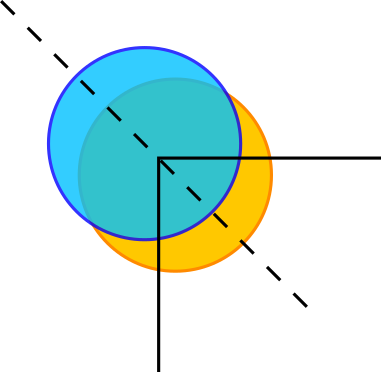
\includegraphics[scale=1.0]{figures/appendix-potential-elastica/distant-disks-1.png}}\\%
\subfloat{
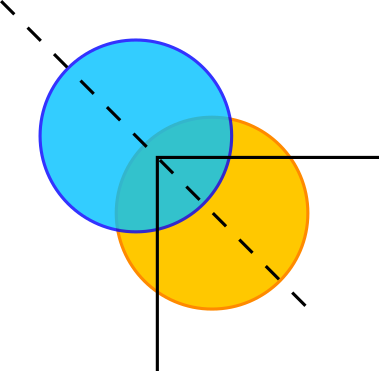
\includegraphics[scale=1.0]{figures/appendix-potential-elastica/distant-disks-2.png}}\\%
\subfloat{
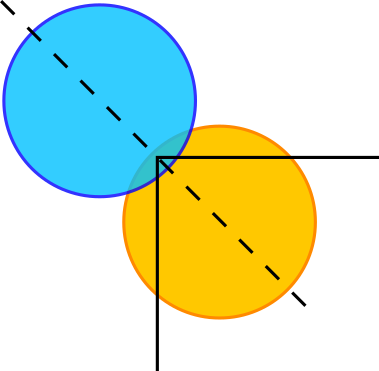
\includegraphics[scale=1.0]{figures/appendix-potential-elastica/distant-disks-3.png}}
\end{minipage}%
\begin{minipage}{0.75\textwidth}
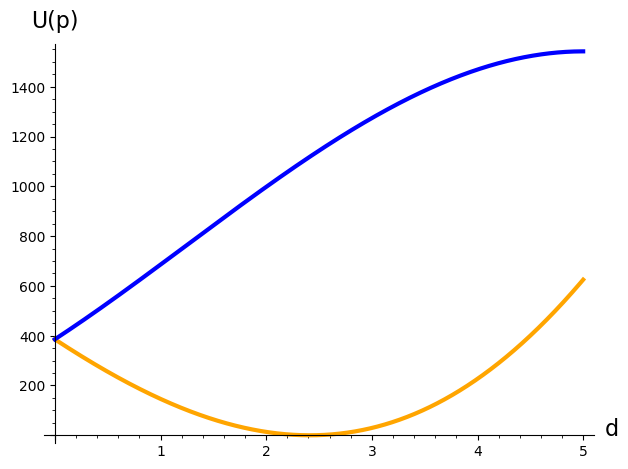
\includegraphics[scale=0.75]{figures/appendix-potential-elastica/potential-elastica-plot.png}
\end{minipage}
\caption{The unbalance difference of equidistant points from the shape contour preserves squared curvature information.}
\label{fig:unbalance-plot}
\end{figure}


In figure \ref{fig:unbalance-plot}, the unbalance grows if the estimation ball is moved towards the exterior and decreases if the estimation ball is moved towards the interior of the shape. That is an indication that we should remove point $p$ from $S$ to decrease the curvature of the shape at point $p \in \partial S$. The same point $p$ may be touched by several balls, each of them contributing with some value for the ultimate decision of keep or remove point $p$ of $S$. The $m$-potential is defined as the sum of these contributions


\begin{definition}{m-potential}
Given digital shape $S$, natural numbers $r>0, m \neq 0$, the \emph{m-potential} at point $p$ is defined as

\begin{align*}
	U_{m}(S,p) &= \sum_{q \in Q_m(p)}{ u(q),}
\end{align*}

where its zone of influence $Q_m(p)$ is defined as

\begin{align*}
	Q_m(p) &= \left\{\; q \in L_m(S) \; | \; p \in B_r(q) \; \right\}.
\end{align*}

\end{definition}

\begin{figure}[h!]
\center
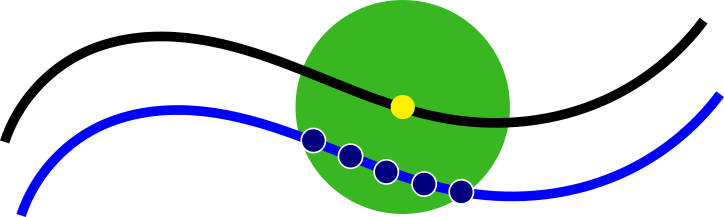
\includegraphics[scale=0.5]{figures/appendix-potential-elastica/k-potential.png}
\caption{The blue points forms the zone of influence of the yellow point.}
\label{fig:unbalance-set}
\end{figure}

The zone of influence of $p$ is the set of all points $q$ in which $p$ is contained in the estimation ball centered at $q$. Finally, we can use the $m$-potential to rewrite the single step FlipFlow energy.


\begin{definition}{$ms$-FlipFlow}
	Given digital shape $X$, we define its $k$-flow as
	
	\begin{align*}
		F_{ms} = \Big\{& S^{(k)} \; | \\
			& S^{(0)} = S,\\
		    &S^{(k+1)} = \argmin \sum_{ x_j \in X_r^{(k)}}{ x_j \Delta _j\big(\; U_{m}(S^{(k)},p) - U_{-m}(S^{(k)},p) \;\big)} - \phi(S^{(k)},m,x_j) \; \Big\},
	\end{align*}
	
	where $\phi(S^{(k)},m,x_j)$ accounts for pairwise terms that were counted twice.
	
	\begin{align*}
	\phi(S^{(k)},m,x_j) = \frac{x_j}{2}\sum_{ x_l \in X_r^{(k)}}{x_l \Delta _{jl}\big(\; U_m(S^{(k)},p) - U_{-m}(S^{(k)},p) \;\big)} 
	\end{align*}
     	  
\end{definition}	

	The inner and outer balls estimates the impact of shifting the center of the ball from a single point in the boundary. That means that limiting the region of influence of each pair of inner and outer balls is important. Each pair of inner and outer balls evaluates the shifting of a single point in the boundary.	
	
	We do not impose any mapping between the inner and outer balls. It will be too complicated otherwise, and we don't need to do it. The mapping is implicitly defined when the inner and outer balls are positioned at $m$-rings with high value of $m$. The larger the value of $m$ the smaller is the zone of influence of each point. In the limit, each pair of balls would touch a single point in the pixel boundary. 
	
	That observation let us to ask if a graph-cut model may be devised for the problem.
	
